% Generated by Sphinx.
\def\sphinxdocclass{report}
\documentclass[letterpaper,10pt,english]{sphinxmanual}
\usepackage[utf8]{inputenc}
\DeclareUnicodeCharacter{00A0}{\nobreakspace}
\usepackage{cmap}
\usepackage[T1]{fontenc}
\usepackage{babel}
\usepackage{times}
\usepackage[Bjarne]{fncychap}
\usepackage{longtable}
\usepackage{sphinx}
\usepackage{multirow}


\title{Open Science Data Cloud Documentation}
\date{April 15, 2013}
\release{1.0}
\author{Tyler Kissinger}
\newcommand{\sphinxlogo}{}
\renewcommand{\releasename}{Release}
\makeindex

\makeatletter
\def\PYG@reset{\let\PYG@it=\relax \let\PYG@bf=\relax%
    \let\PYG@ul=\relax \let\PYG@tc=\relax%
    \let\PYG@bc=\relax \let\PYG@ff=\relax}
\def\PYG@tok#1{\csname PYG@tok@#1\endcsname}
\def\PYG@toks#1+{\ifx\relax#1\empty\else%
    \PYG@tok{#1}\expandafter\PYG@toks\fi}
\def\PYG@do#1{\PYG@bc{\PYG@tc{\PYG@ul{%
    \PYG@it{\PYG@bf{\PYG@ff{#1}}}}}}}
\def\PYG#1#2{\PYG@reset\PYG@toks#1+\relax+\PYG@do{#2}}

\expandafter\def\csname PYG@tok@gd\endcsname{\def\PYG@tc##1{\textcolor[rgb]{0.63,0.00,0.00}{##1}}}
\expandafter\def\csname PYG@tok@gu\endcsname{\let\PYG@bf=\textbf\def\PYG@tc##1{\textcolor[rgb]{0.50,0.00,0.50}{##1}}}
\expandafter\def\csname PYG@tok@gt\endcsname{\def\PYG@tc##1{\textcolor[rgb]{0.00,0.27,0.87}{##1}}}
\expandafter\def\csname PYG@tok@gs\endcsname{\let\PYG@bf=\textbf}
\expandafter\def\csname PYG@tok@gr\endcsname{\def\PYG@tc##1{\textcolor[rgb]{1.00,0.00,0.00}{##1}}}
\expandafter\def\csname PYG@tok@cm\endcsname{\let\PYG@it=\textit\def\PYG@tc##1{\textcolor[rgb]{0.25,0.50,0.56}{##1}}}
\expandafter\def\csname PYG@tok@vg\endcsname{\def\PYG@tc##1{\textcolor[rgb]{0.73,0.38,0.84}{##1}}}
\expandafter\def\csname PYG@tok@m\endcsname{\def\PYG@tc##1{\textcolor[rgb]{0.13,0.50,0.31}{##1}}}
\expandafter\def\csname PYG@tok@mh\endcsname{\def\PYG@tc##1{\textcolor[rgb]{0.13,0.50,0.31}{##1}}}
\expandafter\def\csname PYG@tok@cs\endcsname{\def\PYG@tc##1{\textcolor[rgb]{0.25,0.50,0.56}{##1}}\def\PYG@bc##1{\setlength{\fboxsep}{0pt}\colorbox[rgb]{1.00,0.94,0.94}{\strut ##1}}}
\expandafter\def\csname PYG@tok@ge\endcsname{\let\PYG@it=\textit}
\expandafter\def\csname PYG@tok@vc\endcsname{\def\PYG@tc##1{\textcolor[rgb]{0.73,0.38,0.84}{##1}}}
\expandafter\def\csname PYG@tok@il\endcsname{\def\PYG@tc##1{\textcolor[rgb]{0.13,0.50,0.31}{##1}}}
\expandafter\def\csname PYG@tok@go\endcsname{\def\PYG@tc##1{\textcolor[rgb]{0.20,0.20,0.20}{##1}}}
\expandafter\def\csname PYG@tok@cp\endcsname{\def\PYG@tc##1{\textcolor[rgb]{0.00,0.44,0.13}{##1}}}
\expandafter\def\csname PYG@tok@gi\endcsname{\def\PYG@tc##1{\textcolor[rgb]{0.00,0.63,0.00}{##1}}}
\expandafter\def\csname PYG@tok@gh\endcsname{\let\PYG@bf=\textbf\def\PYG@tc##1{\textcolor[rgb]{0.00,0.00,0.50}{##1}}}
\expandafter\def\csname PYG@tok@ni\endcsname{\let\PYG@bf=\textbf\def\PYG@tc##1{\textcolor[rgb]{0.84,0.33,0.22}{##1}}}
\expandafter\def\csname PYG@tok@nl\endcsname{\let\PYG@bf=\textbf\def\PYG@tc##1{\textcolor[rgb]{0.00,0.13,0.44}{##1}}}
\expandafter\def\csname PYG@tok@nn\endcsname{\let\PYG@bf=\textbf\def\PYG@tc##1{\textcolor[rgb]{0.05,0.52,0.71}{##1}}}
\expandafter\def\csname PYG@tok@no\endcsname{\def\PYG@tc##1{\textcolor[rgb]{0.38,0.68,0.84}{##1}}}
\expandafter\def\csname PYG@tok@na\endcsname{\def\PYG@tc##1{\textcolor[rgb]{0.25,0.44,0.63}{##1}}}
\expandafter\def\csname PYG@tok@nb\endcsname{\def\PYG@tc##1{\textcolor[rgb]{0.00,0.44,0.13}{##1}}}
\expandafter\def\csname PYG@tok@nc\endcsname{\let\PYG@bf=\textbf\def\PYG@tc##1{\textcolor[rgb]{0.05,0.52,0.71}{##1}}}
\expandafter\def\csname PYG@tok@nd\endcsname{\let\PYG@bf=\textbf\def\PYG@tc##1{\textcolor[rgb]{0.33,0.33,0.33}{##1}}}
\expandafter\def\csname PYG@tok@ne\endcsname{\def\PYG@tc##1{\textcolor[rgb]{0.00,0.44,0.13}{##1}}}
\expandafter\def\csname PYG@tok@nf\endcsname{\def\PYG@tc##1{\textcolor[rgb]{0.02,0.16,0.49}{##1}}}
\expandafter\def\csname PYG@tok@si\endcsname{\let\PYG@it=\textit\def\PYG@tc##1{\textcolor[rgb]{0.44,0.63,0.82}{##1}}}
\expandafter\def\csname PYG@tok@s2\endcsname{\def\PYG@tc##1{\textcolor[rgb]{0.25,0.44,0.63}{##1}}}
\expandafter\def\csname PYG@tok@vi\endcsname{\def\PYG@tc##1{\textcolor[rgb]{0.73,0.38,0.84}{##1}}}
\expandafter\def\csname PYG@tok@nt\endcsname{\let\PYG@bf=\textbf\def\PYG@tc##1{\textcolor[rgb]{0.02,0.16,0.45}{##1}}}
\expandafter\def\csname PYG@tok@nv\endcsname{\def\PYG@tc##1{\textcolor[rgb]{0.73,0.38,0.84}{##1}}}
\expandafter\def\csname PYG@tok@s1\endcsname{\def\PYG@tc##1{\textcolor[rgb]{0.25,0.44,0.63}{##1}}}
\expandafter\def\csname PYG@tok@gp\endcsname{\let\PYG@bf=\textbf\def\PYG@tc##1{\textcolor[rgb]{0.78,0.36,0.04}{##1}}}
\expandafter\def\csname PYG@tok@sh\endcsname{\def\PYG@tc##1{\textcolor[rgb]{0.25,0.44,0.63}{##1}}}
\expandafter\def\csname PYG@tok@ow\endcsname{\let\PYG@bf=\textbf\def\PYG@tc##1{\textcolor[rgb]{0.00,0.44,0.13}{##1}}}
\expandafter\def\csname PYG@tok@sx\endcsname{\def\PYG@tc##1{\textcolor[rgb]{0.78,0.36,0.04}{##1}}}
\expandafter\def\csname PYG@tok@bp\endcsname{\def\PYG@tc##1{\textcolor[rgb]{0.00,0.44,0.13}{##1}}}
\expandafter\def\csname PYG@tok@c1\endcsname{\let\PYG@it=\textit\def\PYG@tc##1{\textcolor[rgb]{0.25,0.50,0.56}{##1}}}
\expandafter\def\csname PYG@tok@kc\endcsname{\let\PYG@bf=\textbf\def\PYG@tc##1{\textcolor[rgb]{0.00,0.44,0.13}{##1}}}
\expandafter\def\csname PYG@tok@c\endcsname{\let\PYG@it=\textit\def\PYG@tc##1{\textcolor[rgb]{0.25,0.50,0.56}{##1}}}
\expandafter\def\csname PYG@tok@mf\endcsname{\def\PYG@tc##1{\textcolor[rgb]{0.13,0.50,0.31}{##1}}}
\expandafter\def\csname PYG@tok@err\endcsname{\def\PYG@bc##1{\setlength{\fboxsep}{0pt}\fcolorbox[rgb]{1.00,0.00,0.00}{1,1,1}{\strut ##1}}}
\expandafter\def\csname PYG@tok@kd\endcsname{\let\PYG@bf=\textbf\def\PYG@tc##1{\textcolor[rgb]{0.00,0.44,0.13}{##1}}}
\expandafter\def\csname PYG@tok@ss\endcsname{\def\PYG@tc##1{\textcolor[rgb]{0.32,0.47,0.09}{##1}}}
\expandafter\def\csname PYG@tok@sr\endcsname{\def\PYG@tc##1{\textcolor[rgb]{0.14,0.33,0.53}{##1}}}
\expandafter\def\csname PYG@tok@mo\endcsname{\def\PYG@tc##1{\textcolor[rgb]{0.13,0.50,0.31}{##1}}}
\expandafter\def\csname PYG@tok@mi\endcsname{\def\PYG@tc##1{\textcolor[rgb]{0.13,0.50,0.31}{##1}}}
\expandafter\def\csname PYG@tok@kn\endcsname{\let\PYG@bf=\textbf\def\PYG@tc##1{\textcolor[rgb]{0.00,0.44,0.13}{##1}}}
\expandafter\def\csname PYG@tok@o\endcsname{\def\PYG@tc##1{\textcolor[rgb]{0.40,0.40,0.40}{##1}}}
\expandafter\def\csname PYG@tok@kr\endcsname{\let\PYG@bf=\textbf\def\PYG@tc##1{\textcolor[rgb]{0.00,0.44,0.13}{##1}}}
\expandafter\def\csname PYG@tok@s\endcsname{\def\PYG@tc##1{\textcolor[rgb]{0.25,0.44,0.63}{##1}}}
\expandafter\def\csname PYG@tok@kp\endcsname{\def\PYG@tc##1{\textcolor[rgb]{0.00,0.44,0.13}{##1}}}
\expandafter\def\csname PYG@tok@w\endcsname{\def\PYG@tc##1{\textcolor[rgb]{0.73,0.73,0.73}{##1}}}
\expandafter\def\csname PYG@tok@kt\endcsname{\def\PYG@tc##1{\textcolor[rgb]{0.56,0.13,0.00}{##1}}}
\expandafter\def\csname PYG@tok@sc\endcsname{\def\PYG@tc##1{\textcolor[rgb]{0.25,0.44,0.63}{##1}}}
\expandafter\def\csname PYG@tok@sb\endcsname{\def\PYG@tc##1{\textcolor[rgb]{0.25,0.44,0.63}{##1}}}
\expandafter\def\csname PYG@tok@k\endcsname{\let\PYG@bf=\textbf\def\PYG@tc##1{\textcolor[rgb]{0.00,0.44,0.13}{##1}}}
\expandafter\def\csname PYG@tok@se\endcsname{\let\PYG@bf=\textbf\def\PYG@tc##1{\textcolor[rgb]{0.25,0.44,0.63}{##1}}}
\expandafter\def\csname PYG@tok@sd\endcsname{\let\PYG@it=\textit\def\PYG@tc##1{\textcolor[rgb]{0.25,0.44,0.63}{##1}}}

\def\PYGZbs{\char`\\}
\def\PYGZus{\char`\_}
\def\PYGZob{\char`\{}
\def\PYGZcb{\char`\}}
\def\PYGZca{\char`\^}
\def\PYGZam{\char`\&}
\def\PYGZlt{\char`\<}
\def\PYGZgt{\char`\>}
\def\PYGZsh{\char`\#}
\def\PYGZpc{\char`\%}
\def\PYGZdl{\char`\$}
\def\PYGZhy{\char`\-}
\def\PYGZsq{\char`\'}
\def\PYGZdq{\char`\"}
\def\PYGZti{\char`\~}
% for compatibility with earlier versions
\def\PYGZat{@}
\def\PYGZlb{[}
\def\PYGZrb{]}
\makeatother

\begin{document}

\maketitle
\tableofcontents
\phantomsection\label{index::doc}


Contents:


\chapter{Introduction to the Open Science Data Cloud}
\label{intro::doc}\label{intro:introduction-to-the-open-science-data-cloud}\label{intro:welcome-to-open-science-data-cloud-s-documentation}
The \href{https://opensciencedatacloud.org}{Open Science Data Cloud} is a distributed, cloud-based infrastructure for managing, analyzing, archiving and sharing scientific datasets.


\section{``Big-Picture'' Diagram of OSDC Infrastructure}
\label{intro:big-picture-diagram-of-osdc-infrastructure}
The Open Science Data Cloud is currently composed two cloud systems: \textbf{Adler}, based on \href{http://www.eucalyptus.com/eucalyptus-cloud/iaas}{Eucalyptus}; and \textbf{Sullivan}, based on \href{http://www.openstack.org/}{OpenStack}.

\scalebox{0.450000}{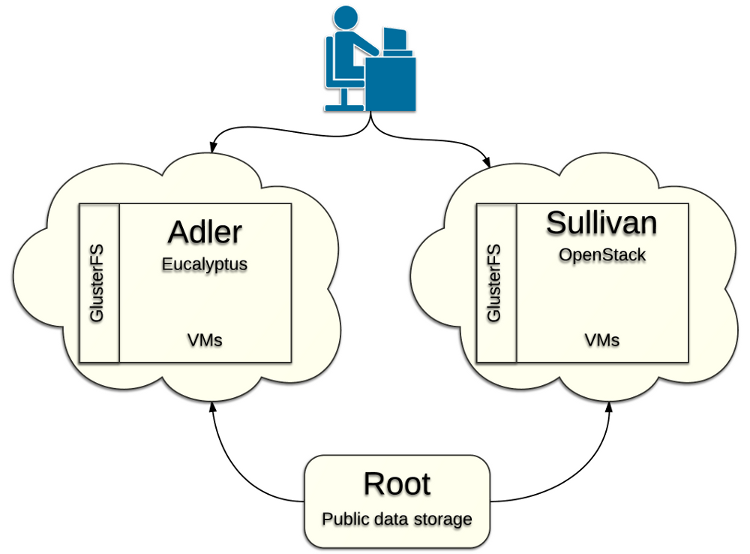
\includegraphics{images/OSDCinfrastructure.png}}

\code{Internet (users)}

\code{ssh -A login1.opensciencedatacloud.org (Adler)} or \code{ssh -A login2.opensciencedatacloud.org (Sullivan)}

\code{Open Science Data Cloud (VMs) -{-}\textgreater{}-{-} NAT -{-}\textgreater{}-{-} Internet}

\code{GlusterFs/CIFS (shared filesystem)}


\chapter{Getting Started with the Open Science Data Cloud}
\label{gettingstarted::doc}\label{gettingstarted:getting-started-with-the-open-science-data-cloud}

\section{Who should apply for an OSDC Account?}
\label{gettingstarted:who-should-apply-for-an-osdc-account}
The OSDC is intended to provide resources for scientists and researchers that are working on data-intensive projects...


\section{Requesting an OSCD Account}
\label{gettingstarted:requesting-an-oscd-account}
To request an account on the OSDC, please visit the \href{https://www.opensciencedatacloud.org/apply/}{Account Application page} and provide the necessary information.


\subsection{Key Generation}
\label{gettingstarted:key-generation}
To apply for an account on the OSDC, you must provide an SSH public key. This key will allow you to connect to the login server through a Secure Shell (SSH). The SSH public key is one half of a SSH keypair, which is for secure interactions between two networked computers.


\subsubsection{On UNIX}
\label{gettingstarted:on-unix}
On a UNIX machine (a machine running Linux, Mac OS X, etc.) open Terminal. Enter (with your own email address):
\begin{quote}

\code{ssh-keygen -t rsa -C "youremail@yourdomain.ext"\textbackslash{}}
\end{quote}

You will be prompted to enter a filename; if the default presented is \code{id\_rsa}, just press enter to accept. If the default presented is not that name, it may be because another file by that name already exists. Check the the \textasciitilde{}/.ssh directory, and if this is the case, you should back up the existing \code{id\_rsa} file. After checking and backing up if the file already existed, enter \code{id\_rsa} for the filename of the new keypair you are generating. You will then be prompted for a passphrase. After entering a passphrase for the key, your public-private keypair will have been generated.

Now, you must copy the \emph{public} key to a plain text file to upload on the Account Application page. It is important to note that you should \textbf{never} share your private key with another party; sharing is what the public key is for. Sharing your private key could allow others to maliciously access systems that you trust. If you are using Mac OS X, to copy your public key to your clipboard, enter:
\begin{quote}

\code{pbcopy \textless{} \textasciitilde{}/.ssh/id\_rsa.pub}
\end{quote}

Or on Linux:
\begin{quote}

\code{sudo apt-get install xclip}

\code{xclip -sel clip \textless{} \textasciitilde{}/.ssh/id\_rsa.pub}
\end{quote}

Now, just create a text file, paste the key into the file, and upload that file on the Account Application page.


\subsubsection{On Windows}
\label{gettingstarted:on-windows}
On a Windows machine, download and install \href{http://www.chiark.greenend.org.uk/~sgtatham/putty/}{PuTTY}, an SSH protocol client program for Windows. Navigate to the Start menu, and under the PuTTY submenu open the PuTTYgen program. Press Generate
..more to be added here


\section{OSDC Monthly Maintenance}
\label{gettingstarted:osdc-monthly-maintenance}
Monthly maintenance will take place on the last Tuesday of each month at 0900CT. Please make sure to save your work and shutdown all instances by that time. A reminder will be sent each month.


\section{Connecting to the OSDC}
\label{gettingstarted:connecting-to-the-osdc}
Connection to the OSDC can be done through two ways: connection through a Secure Shell (SSH), or connection through the Console.


\subsection{Connecting through SSH}
\label{gettingstarted:connecting-through-ssh}
{\scalebox{0.300000}{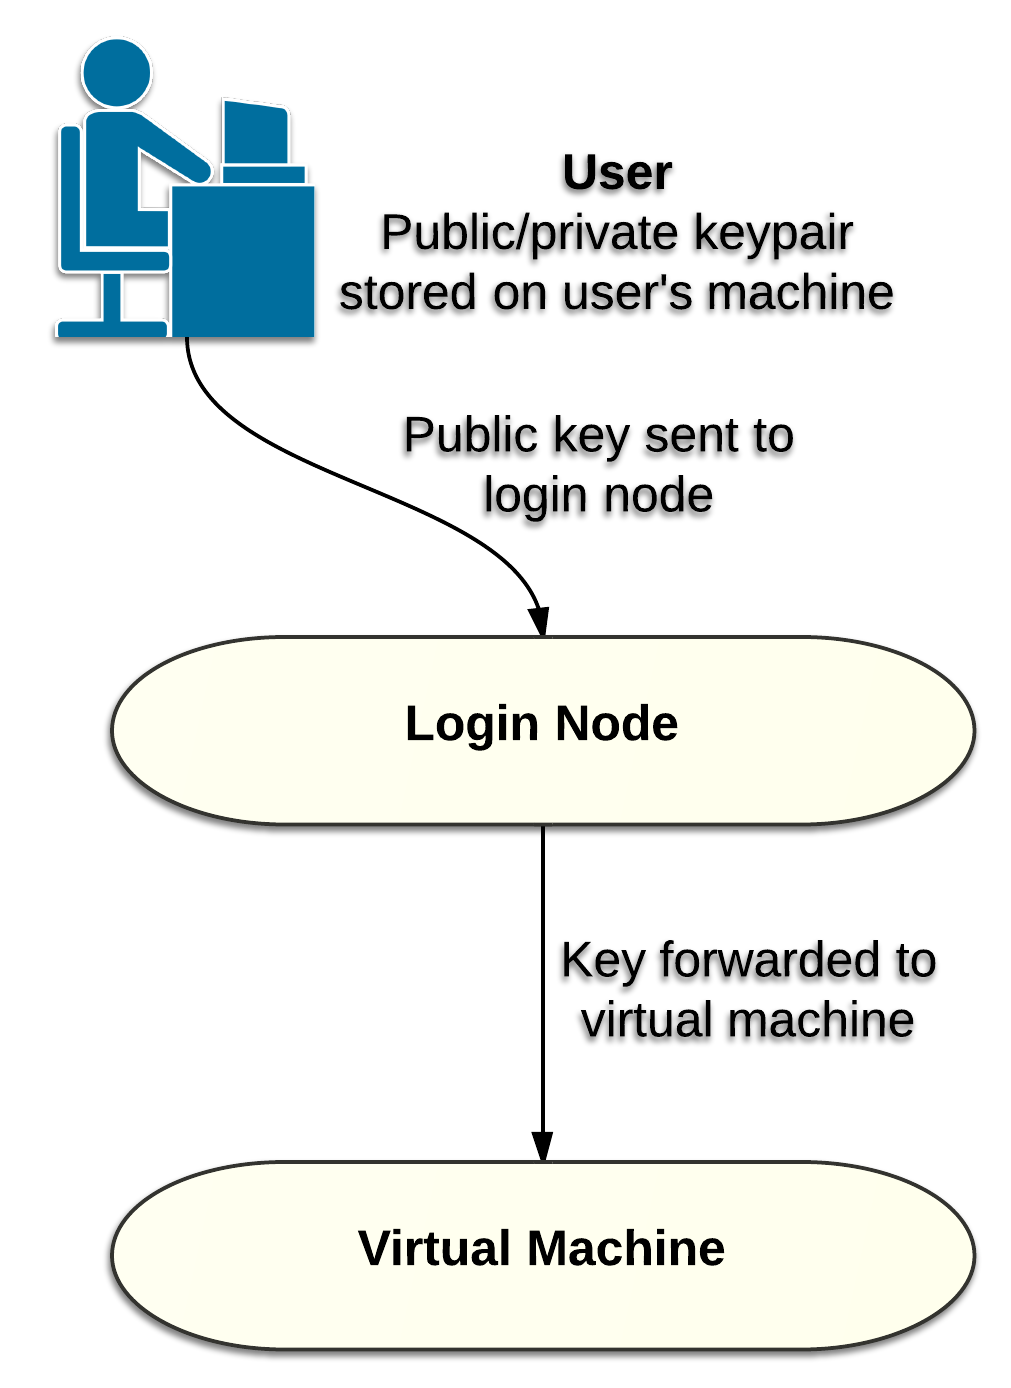
\includegraphics{images/keyforwarding.png}}\hfill}

Secure Shell (SSH) is a network protocol that allows for secure communication between two networked computers over an unsecured network (e.g., the Internet). It is the protocol that is used to connect to the OSDC through a command line interaface. The method for connecting depends on the operating system of the machine you are using.


\subsubsection{SSH on a UNIX Machine}
\label{gettingstarted:ssh-on-a-unix-machine}
To connect to the login server from a UNIX machine, open the Terminal and enter:
\begin{quote}

\code{ssh -A username@login2.opensciencedatacloud.org}
\end{quote}

Including \code{-A} allows for \href{http://www.unixwiz.net/techtips/ssh-agent-forwarding.html}{agent forwarding}; it is necessary because it will allow the server to forward your credentials to the virtual machine (VM). See figure above. If it is not included, you will get an error when you attempt to connect to the VM. You will be prompted for a passphrase; this will be the passphrase you selected when generating the key. Enter it.


\subsubsection{SSH on Windows}
\label{gettingstarted:ssh-on-windows}
To connect to the login server from a Windows machine,


\subsection{Connection through the Console}
\label{gettingstarted:connection-through-the-console}
The OCDC allows two options for login through the Console; Shibboleth and OpenID. If you have an account with a college or university, select \code{Shibboleth} and then select your institution. Enter and submit your credentials associated with that account (\emph{not} your OSDC account). If you don't have an account with a college or university, enter your OpenID credentials to gaina ccess to the Console.

After logging in, it is necessary to establish an SSH keypair for your work on the OSDC. Navigate to the ``Access \& Control'' page. Now, select ``Import Keypair.'' Enter a name for the keypair (traditionally firstinitiallastname), and then copy and paste your public key as described above ({\color{red}\bfseries{}*}hyperlink). Select ``All resources'' from the drop-down menu, and press submit. This will have established a keypair for use by the OSDC.


\section{Workflow}
\label{gettingstarted:workflow}
ssh to the login server

start a VM

ssh to VM

mount shared filesystem with own credentials

…compute!…

when all done, stop your VM


\chapter{Open Science Data Cloud Basic Usage}
\label{basicusage:open-science-data-cloud-basic-usage}\label{basicusage::doc}
In your home directory on the login server (login1.opensciencedatacloud.org), there is a .euca subdirectory containing your EC2 (eucalyptus) credentials. This directory has mode 700 as it contains cryptographic keys for accessing EC2. Keep it protected.

To list images, run:
\begin{quote}

\code{euca-describe-images}
\end{quote}

Look for entries with an ID starting with ‘emi-\emph{’ or ‘ami-}’. OSDC-provided prototypical images are owned by admin and start with ‘prototypical-’.

Following types of VMs are supported:

\begin{tabulary}{\linewidth}{|L|L|L|L|}
\hline
\textbf{
VM Type
} & \textbf{
Cores
} & \textbf{
RAM (MB)
} & \textbf{
Disk (GB)
}\\\hline

m1.small
 & 
1
 & 
3584
 & 
20
\\\hline

m1.large
 & 
2
 & 
716
 & 
20
\\\hline

c1.medium
 & 
4
 & 
14336
 & 
20
\\\hline

m1.xlarge
 & 
8
 & 
28672
 & 
20
\\\hline

c1.xlarge
 & 
8
 & 
28672
 & 
20
\\\hline
\end{tabulary}


To check the cloud availability/usage on the Adler cloud:
\begin{quote}

\code{euca-cloud-status}
\end{quote}

To start an instance on Adler run:
\begin{quote}

\code{euca-run-instances -k USERNAME -n 1 -t m1.small emi-ID}
\end{quote}

To start an instance on Sullivan run:
\begin{quote}

\code{euca-run-instances -k USERNAME -n 1 -t m1.small -f \textasciitilde{}/.smbpasswd.sh emi-ID}
\end{quote}

This will start an m1.small instance as defined by the command above. Note that it is best to start one instance at a time. That is, if one needs 20 instances, they should be started one-at-a-time followed by a delay and then the next instance, until all 20 are running. This effectively resolves Eucalyptus software scalability issues.

To monitor/list instances of one’s group (only!), run:
\begin{quote}

\code{euca-describe-instances}
\end{quote}

This will return status of instances, with instance ID and an instance IP address.

To login to an instance on Adler run:
\begin{quote}

\code{ssh root@INSTANCE\_IP}
\end{quote}

To login to an instance on Sullivan run:
\begin{quote}

\code{ssh ubuntu@INSTANCE\_IP}
\end{quote}

To mount shared filesystem on Adler instances, run following command upon logging in:
\begin{quote}

\code{/cloudconf/mount-glusterfs USERNAME}
\end{quote}

and enter your password.

For Sullivan instances the option -f \textasciitilde{}/smbpasswd.sh ensures the shared filesystem is automatically mounted.

To check output log of an instance, run:
\begin{quote}

\code{euca-get-console-output INSTANCE\_ID}
\end{quote}

To stop an instance, log out of the instance and run this command:
\begin{quote}

\code{euca-terminate-instances INSTANCE\_ID}
\end{quote}


\section{Open Science Data Cloud Image Features}
\label{basicusage:open-science-data-cloud-image-features}
Package installation:
OSDC Adler images are based on GNU/Debian 5.0 ‘Lenny’ amd64 Linux distribution. These images are pre configured to use our lab repository Debian cache service.
OSDC Sullivan images are based on UEC cloud images with Ubuntu 12.04 ‘Precise’.

To find package names, run:
\begin{quote}

\code{apt-cache search KEYWORD1 KEYWORKD2 …}
\end{quote}

To examine package info, run:
\begin{quote}

\code{aptitude show PACKAGENAME}
\end{quote}

To install a package, run:
\begin{quote}

\code{aptitude install -PV PACKAGE-NAME1 PACKAGE-NAME2}
\end{quote}


\section{Creating Open Science Data Cloud images from an Adler instance}
\label{basicusage:creating-open-science-data-cloud-images-from-an-adler-instance}
These instructions only apply to the Adler cloud. Please see below for Sullivan instructions.
\begin{quote}

\code{/cloudconf/mkimage-wrapper}
\end{quote}

Make sure to use a unique image filename \textbf{every} time.

Copy your .euca/ directory from the login1.opensciencedatacloud.org server to the instance. On the login server run:
\begin{quote}

\code{rsync -avu .euca root@INSTANCE\_IP:} (\emph{Be sure to include the colon})
\end{quote}

Source euca env (inside running VM):
\begin{quote}

\code{source \textasciitilde{}/.euca/eucarc}
\end{quote}

Bundle the image:
\begin{quote}

\code{euca-bundle-image -d /scratch/ -i /scratch/"new-unique-name-DATE-ENUM"}
\end{quote}

Upload the bundle:
\begin{quote}

\code{euca-upload-bundle -b BUCKET\_NAME -m /scratch/"new-unique-name-DATE-ENUM".manifest.xml}
\end{quote}
\begin{description}
\item[{Register the image:}] \leavevmode
\code{euca-register BUCKET\_NAME/"new-unique-name-DATE-ENUM".manifest.xml}

\item[{Check if available:}] \leavevmode
\code{euca-describe-images}

\end{description}

Make sure to make a copy your MY-UPDATED-VM.img.manifest.xml file to the login1.opensciencedatacloud.org server, in order to easily remove an image at a later time. On the login server run:
\begin{quote}

\code{rsync -avu root@INSTANCE\_IP:/scratch/"new-unique-name-DATE-ENUM".manifest.xml .}
\end{quote}

To remove images (at a later time):
\begin{quote}

\code{euca-deregister emi-ID}

\code{euca-delete-bundle -b BUCKET\_NAME -m ./"new-unique-name-DATE-ENUM".manifest.xml}
\end{quote}


\section{Creating Open Science Data Cloud images from a Sullivan instance}
\label{basicusage:creating-open-science-data-cloud-images-from-a-sullivan-instance}
These instructions only apply to the Sullivan cloud. Please see above for Adler instructions.

Use the nova client to find the instance ID:
\begin{quote}

\code{nova list}
\end{quote}

Then create the image:
\begin{quote}

\code{nova image-create INSTANCE\_ID new-unique-name-DATE-ENUM}
\end{quote}

By default these images are private and can only be seen by you. To make images public:
\begin{quote}

\code{glance update INSTANCE\_ID is\_public=true}
\end{quote}


\chapter{Indices and tables}
\label{index:indices-and-tables}\begin{itemize}
\item {} 
\emph{genindex}

\item {} 
\emph{modindex}

\item {} 
\emph{search}

\end{itemize}



\renewcommand{\indexname}{Index}
\printindex
\end{document}
